\documentclass{article}
\usepackage[utf8]{inputenc}

\title{Interacting Particle System Thesis}
\author{Stefan Eng}
\date{2019/2020}

\usepackage{amsthm}
\usepackage{amssymb}
\usepackage{amsmath}
\usepackage{hyperref}
\usepackage{caption}
\usepackage{mathrsfs}
\usepackage{blkarray}

\usepackage{natbib}
\usepackage{graphicx}

\usepackage{tikz}
\usetikzlibrary{calc, automata, chains, arrows.meta, graphs, graphs.standard}


\theoremstyle{plain}
\newtheorem{theorem}{Theorem}[section]
\newtheorem{example}{Example}[theorem]
\newtheorem{lemma}[theorem]{Lemma}
\newtheorem{prop}[theorem]{Proposition}
\newtheorem{cor}{Corollary}[theorem]

\theoremstyle{definition}
\newtheorem{defn}[theorem]{Definition}
\newtheorem{exercise}{Exercise}

\theoremstyle{remark}
\newtheorem*{note}{Note}
\newtheorem*{remark}{Remark}

\newcommand{\R}{\mathbb{R}}
\newcommand{\Rs}{\mathcal{R}}
\newcommand{\Gs}{\mathcal{G}}
\newcommand{\Cs}{\mathcal{C}}
\newcommand{\Q}{\mathbb{Q}}
\newcommand{\A}{\mathcal{A}}
\newcommand{\F}{\mathcal{F}}
\newcommand{\E}{\mathcal{E}}
\newcommand{\M}{\mathcal{M}}
\newcommand{\N}{\mathcal{N}}
\newcommand{\Z}{\mathbb{Z}}
\newcommand{\Zs}{{\{0,1\}^\mathbb{Z}}}
\newcommand{\I}{\mathcal{I}}
\newcommand{\D}{\mathcal{D}}
\newcommand{\B}{{\mathcal{B}_{\mathbb{R}}}}
\newcommand{\BU}{{\mathcal{B}_{[0,1]}}}
\newcommand{\loc}{L_{\text{loc}}^1}
\newcommand{\powset}{\mathcal{P}}
\newcommand{\outm}{\mu^{*}}
\newcommand{\cdict}{\Rightarrow\!\Leftarrow}
\newcommand{\Var}{\operatorname {Var}}

% X_1, ..., X_n
\newcommand{\Xn}{\ensuremath{X_1,\ldots,X_n}}
\newcommand{\xn}{\ensuremath{x_1,\ldots,x_n}}

\begin{document}

\maketitle

\section{Background}

\subsection{Probability}

\begin{defn}[Exponential Distribution]
Let $X$ be a random variable.
If $X$ has a pdf of 
$$
f(x) = \begin{cases}
    \lambda e^{-\lambda x} & x > 0\\
    0 & x \leq 0
    \end{cases}
$$
then we say that $X$ is exponentially distributed with rate $\lambda$ (denoted as $X \sim \exp(\lambda)$.
\end{defn}

\begin{theorem}\label{thm:exp_x_less_y}
Let $X \sim \exp(\alpha)$ and $Y \sim \exp(\beta)$ be independent random variables.
Then 
$$
P(X < Y) = \frac{\alpha}{\alpha + \beta}
$$
\end{theorem}

\begin{proof}
\begin{align*}
    P(X < Y) &= \int_0^\infty P(X < y | Y = y) f_Y(y) dy\\
    &= \int_0^\infty (1 - e^{-\alpha y}) \beta e^{-\beta y} dy\\
    &= \beta \int_0^\infty \left( e^{-\beta y} - e^{-(\alpha + \beta) y}\right) dy\\
    &= \beta \left(\frac{1}{\beta} - \frac{1}{\alpha + \beta}\right)\\
    &= \frac{\alpha}{\alpha + \beta}
\end{align*}
\end{proof}

\begin{theorem}\label{thm:exp_t_cond}
Let $X \sim \exp(\alpha)$ and $Y \sim \exp(\beta)$ be independent random variables with $T = \min(X,Y)$
Then $T \sim \exp(\alpha + \beta)$.
\end{theorem}

\begin{proof}
\begin{align*}
    P(\min(X,Y) > z) &= P(X > z, Y > z)\\
    &= P(X > z) P(Y > z)\\
    &= e^{-\alpha z} e^{-\beta z}\\
    &= e^{-(\alpha + \beta) z}
\end{align*}
So $\min(X,Y) = T \sim \exp(\alpha + \beta)$
\end{proof}

\begin{theorem} \label{thm:exp_scaling}
Let $X \sim \exp(\lambda)$ and $c$ be a constant.
Then $cX \sim \exp(\lambda/c)$.
\end{theorem}

\begin{proof}
$$
    P(cX > y) = P(X > y/c) = e^{-\lambda/c y}
$$
So $cX \sim \exp(\lambda/c)$ 
\end{proof}

\subsubsection{Generating functions and Characteristic Functions}

\begin{defn}[Probability generating function]
The probability generating function of a discrete random variable $X \in \{0,1,2, \ldots\}$ is defined as $G_X(z) = E[z^X] = \sum_{i = 0}^\infty z^i P(X = i)$.
\end{defn}

\begin{lemma}
For discrete random variable $X$,
\begin{itemize}
    \item $G_X(0) = P(X = 0)$
    \item $G_X(1) = 1$
\end{itemize}
\end{lemma}

\begin{defn}[Characteristic function]
The characteristic function of a random variable $X$ is $\varphi_X(t) = E[e^{itX}]$
\end{defn}

\begin{theorem}[Moments from generating function] \cite{grimmett2001}
Let $X$ be a random variable and $G_X(z)$ be its generating function
\begin{itemize}
    \item $E[X] = G'(1)$
    \item $E[X (X - 1) \cdots (X - k + 1)] = G^{(k)}(1)$
\end{itemize}
\end{theorem}

\begin{proof}
See \cite{grimmett2001}
\end{proof}

\begin{theorem}
If $X$ and $Y$ are independent discrete random variables then
$$
G_{X + Y}(z) = G_X(z) G_Y(z)
$$

For any random variables $X$ and $Y$, 
$$
\varphi_{X + Y}(t) = \varphi_X(t) \varphi_Y(t)
$$
\end{theorem}

\begin{proof}
See \cite{grimmett2001}
\end{proof}



\begin{theorem}\label{thm:generating_random_sum}
Let $X_1, X_2, \ldots$ be iid random variables with common probability generating function $G_X(t)$.
Let $N$ be another non-negative integer random variable, independent of the sequence $(X_t)$.
Let $G_N(z) = E[z^N]$ and $G_X(z)$ be the probability generating functions for $N$ and each $X_i$.
Let $S = \sum_{i = 1}^N X_i$.
Then,
$$
G_S(z) = G_N(G_X(z))
$$
\end{theorem}

\begin{proof}
\begin{align*}
    G_X(z) &= E[ z^S ]\\
    &= E[ E[ z^{\sum_{i = 1}^N X_i} | N ]]\\
    &= E \left[ \prod_{i = 1}^N E[z^{X_i} | N] \right] && \text{by independence}\\
    &= E \left[ \prod_{i = 1}^N E[z^{X_i}] \right]\\
    &= E[ G_X(z)^N]\\
    &= G_N(G_X(z))
\end{align*}
\end{proof}

\begin{theorem}\label{thm:char_func_random_sum}
Let $X_1, X_2, \ldots$ be iid random variables with common characteristic function $\varphi_X(t)$.
Let $N$ be another non-negative integer random variable, independent of the sequence $(X_t)$.
Let $G_N(z) = E[z^N]$ be the probability generating function for $N$.
Let $S = \sum_{i = 1}^N X_i$.
Then,
$$
\varphi_S(t) = E[\varphi_X(t)^N] = G_N(\varphi_X(t))
$$
\end{theorem}

\begin{proof}
\begin{align*}
    \varphi_S(t) &= E[ \exp(it \sum_{i = 1}^N X_i) ]\\
    &= E[ E[ \exp(it \sum_{i = 1}^N X_i) | N ]]\\
    &= E \left[ \prod_{i = 1}^N E[\exp(it X_i) | N] \right] && \text{by independence}\\
    &= E[\varphi_X(t)]\\
    &= G_N(\varphi_X(z))
\end{align*}
\end{proof}

\subsubsection{Random Sums}

\begin{theorem} \label{thm:geom_sum_exp}
Let $N$ be geometrically distributed with parameter $p$.
$P(N = n) = (1 - p)^{n - 1} p$ and $X_1,X_2,\ldots$ iid and independent of $N$ with each $X_i$ exponentially distributed with rate $\lambda$.
Then,
$$
S = \sum_{i = i}^N X_i
$$
has an exponential distribution with rate $p \lambda$.
\end{theorem}

\begin{proof}
Let $G_N(z)$ be the probability generating function of $N$ and $\varphi_X(t)$ be the characteristic function of each $X_i$.
\begin{align*}
    G_N(z) &= \frac{pz}{1 - (1 - p)z}\\
    \varphi_X(t) &= \frac{\lambda}{\lambda - it}
\end{align*}
Then by Theorem \ref{thm:char_func_random_sum},
\begin{align*}
    \varphi_S(t) &= G_N(\varphi_X(t))\\
    &= \frac{
        p \left( \frac{\lambda}{\lambda - it} \right)
        } {
        1 - (1 - p) \frac{\lambda}{\lambda - it}
        }\\
    &= \frac{ 
        p \lambda
    } {
        \lambda - it - \lambda + p \lambda
    }\\
    &= \frac{ 
        p \lambda
    } {
        p \lambda - it 
    }
\end{align*}
Which is the characteristic function of the exponential distribution with rate $p \lambda$.
\end{proof}

\begin{theorem}[Wald's equation]\label{thm:random_sum_ev} \cite{Ross97}
Let $X_1, X_2, \ldots$ be sequence of iid random variables and $N$ a non-negative integer random variable independent of the sequence $(X_n)$.
Let $S = \sum_{i = 1}^N X_i$
Then,
$$
E[ S ] = E\left[\sum_{i = 1}^N X_i\right] = E[X] E[N]
$$
\end{theorem}

\begin{proof}
Let $G_N(z)$ and $G_X(z)$ be the probability generating functions for $N$ and each $X_i$.
By Theorem \ref{thm:generating_random_sum}, we have that $G_S(z) = G_N(G_X(z))$.
Hence,
$G'_S(z) = G'_N(G_X(z)) \cdot G'_X(z)$.
By properties of the probability generating function, we have that
\begin{align*}
    E[S] &= G'_S(1)\\
    &= G'_N(G_X(1)) \cdot G'_X(1)\\
    &= G'_N(1) G'_X(1)\\
    &= E[N] E[X]
\end{align*}

% The not as elegant way.
%\begin{align*}
%    E\left[ \sum_{i = 1}^N X_i \right] &= E\left[ E\left[ \sum_{i = 1}^N X_i | N\right] \right]\\
%    &= \sum_{n = 1}^\infty E\left[ \sum_{i = 1}^n X_i \right] P(N = n) && N, (X_t) \text{ indep.}\\
%    &= \sum_{n = 1}^\infty \sum_{i = 1}^n E\left[ X_i \right] P(N = n)\\
%    &= E\left[ X_i \right] \sum_{n = 1}^\infty n \cdot P(N = n)\\
%    &= E[X_i] E[N]
%\end{align*}
\end{proof}

\begin{theorem} \label{thm:random_sum_var}
Let $X_1, X_2, \ldots$ be iid random variables and $N$ a non-negative integer random variable independent of each $X_i$.
Then,
$$
\Var\left( \sum_{i = 1}^N X_i \right) = E[N]\Var(X) + (E[X])^2 \Var(N)
$$
\end{theorem}

\begin{proof}
TODO
\end{proof}

\begin{theorem}\label{thm:geom_sum_geom}
Let $X_1, X_2, \ldots$ be iid geometric random variables ($X_i \in \{1,2,\ldots\})$, with parameters $p$ and $N$ a geometric random variable ($N \in \{1,2,\ldots\})$ with parameter $\alpha$, independent of the sequence $(X_t)$.
Then,
$$
S = \sum_{i = 1}^N X_i
$$
is geometrically distributed with parameter $\alpha p$.
\end{theorem}

\begin{proof}\cite{Nelson1995}
The probability generating functions for $N$ and each $X_i$ are
\begin{align*}
    G_X(z) &= \frac{p z}{1 - (1 - p)z}\\
    G_{N}(z) &= \frac{\alpha z}{1 - (1 - \alpha)z}
\end{align*}

It follows that
\begin{align*}
    G_S(z) &= G_N(G_X(z))\\
    &= \frac{
    \alpha \left( \frac{p z}{1 - (1 - p)z} \right)
    }{
        1 - (1 - \alpha) \left( \frac{p z}{1 - (1 - p)z} \right)
    }\\
    &= \frac{
        \alpha p z
    }{
        1 - z + pz - pz + \alpha p z
    } \\
    &= \frac{
        \alpha p z
    }{
        1 - (1 - \alpha p) z
    }
\end{align*}
So $S$ is geometrically distributed with parameter $\alpha p$
\end{proof}

\subsection{Markov Chains}

\begin{defn}[Canonical Form] \cite{grinstead2003}
Assume we have a absorbing Markov chain with $r$ absorbing states and $t$ transient states and  transition matrix $P$.
The canonical form of the transition matrix is
\begin{equation}
    P = \begin{pmatrix}
        Q & R\\
        0 & I_{r}
    \end{pmatrix}
\end{equation}

where $Q$ is an $r \times r$ matrix of transient states, $R$ is an $t \times t$ matrix of absorbing states and $I_{r}$ is the $r \times r$ identity matrix.
\end{defn}

\begin{theorem} \label{thm:fund_exp} \cite{grinstead2003}
For an absorbing Markov chain the expected number of times that a chain is given by
\begin{equation}
    N = I + Q + Q^2 + \cdots = (I - Q)^{-1}
\end{equation}
Where $Q$ is the $Q$ is an $r \times r$ matrix of transient states from the canonical form.
$N_{ij}$ is the expected number of times the chain is in state j when starting in state i.
\end{theorem}

\begin{proof}
See \cite{grinstead2003}
\end{proof}

\begin{theorem}\label{thm:mc_projection} \cite{LevinPeresWilmer2006}
Let $(X_t)$ be a Markov chain with state space $\Omega$ and transition matrix $P$.
Let $\sim$ be an equivalence relation on $\Omega$ and denote the equivalences classes as $\Omega' = \{[x]: x \in \Omega\}$.

If $x \sim x'$ implies that $P(x,[y]) = P(x', [y])$ then $[X_t]$  is a Markov chain.
The state space is the equivalence classes $\Omega'$ and transition matrix $P'$ defined as $P'([x],[y]) := P(x, [y])$
\end{theorem}

\section{Contact Process on Finite Graphs}

Now we look at a contact process on a finite graph.
Based on finite Markov chain theory, no matter the initial state, the process will eventually be zero.
We look at $T_\lambda$, the time until we reach the state zero while keeping the number of nodes fixed as $\lambda$ goes to $\infty$.
First we investigate the behavior for a complete graph, in which each node is connected to all other nodes and then we look at the one-dimensional lattice, in which each node is connected to at most two neighbors.

\begin{defn}[Contact process]
Let $X = \{0,1\}^S$ be a finite state space.
\end{defn}

\subsection{Two node contact process}

Define a contact process on the finite graph with two nodes and one edge between them.

\begin{align}
    1 &\to 0 \text{ at rate } 1\\
    0 &\to 1 \text{ at rate } \begin{cases}
        \lambda & \text{ if neighbor is 1}\\
        0 & \text{ otherwise}
    \end{cases}
\end{align}

Start the process with both nodes at 1.
Clearly we will eventually reach $(0,0)$.
We can express the transition rate matrix $Q$ matrix as

% Info on blockarray
% https://tex.stackexchange.com/a/59519/41827
$$
Q = \begin{blockarray}{ccccc}
    & (1,1) & (1,0) & (0,1) & (0,0)\\
    \begin{block}{c(cccc)}
        (1,1) & -2 & 1 & 1 & 0\\
        (1,0) & \lambda & - 1 - \lambda & 0 & 1\\
        (0,1) & \lambda & 0 & - 1 - \lambda & 1\\
        (0,0) & 0 & 0 & 0 & 0\\
    \end{block}
\end{blockarray}
$$

We can project this Markov chain to the number of ones in the process at a given time.
That is, mapping $\{(1,0),(0,1)\}$ to a single state 1.
This new chain is also a Markov chain by Theorem \ref{thm:mc_projection}.

$$
Q = \begin{blockarray}{cccc}
    & 2 & 1 & 0\\
    \begin{block}{c(ccc)}
        2 & -2 & 2 & 0\\
        1 & \lambda & - 1 - \lambda & 1\\
        0 & 0 & 0 & 0\\
    \end{block}
\end{blockarray}
$$

\begin{figure}
    \centering
   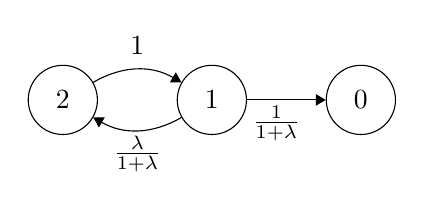
\begin{tikzpicture}[start chain = going right,
   -Triangle, every loop/.append style = {-Triangle}]
   \node[state, on chain]  (2) {2};
   \node[state, on chain]  (1) {1};
   \node[state, on chain]  (0) {0};
   
   % TODO: Need to add labels
   \draw (2) edge[bend left] node[yshift=3mm]{$1$} (1);
   \draw (1) edge[bend left] node[yshift=-3mm]{$\frac{\lambda}{1 + \lambda}$}(2);
   \draw (1) edge[left] node[xshift=3mm, yshift=-3mm]{$\frac{1}{1 + \lambda}$} (0);
   
\end{tikzpicture}
    \caption{Projected embedded discrete Markov chain for two node contact process}
    \label{fig:discrete_mc_two_contact}
\end{figure}

Let $T_\lambda$ be the time in which we hit 0.
The waiting time while in state 2 is exponentially distributed random variable $X$ with parameter $- q_{2} = 2$ and similarly the waiting time while in state 1 is exponentially distributed with parameter $- q_{(1,0)} = 1 + \lambda$.

Let $N$ be a geometric random variable which denotes the number of times that the process waits at state 1 before moving to the absorbing state 0.
$$
P(N = n) = \left(\frac{\lambda}{1 + \lambda} \right)^{n - 1} \frac{1}{1 + \lambda} \quad n = 1,2,\ldots
$$
with
\begin{align*}
    E[N] &= 1 + \lambda\\
    \Var(N) &= \frac{\lambda/(1 + \lambda)}{1/(1 + \lambda)^2} = \lambda (1 + \lambda)
\end{align*}

Let $X_1, X_2, \ldots$ be iid random variables with
$X_i \sim \exp(2)$ for the waiting time at state 2 and independent of iid random variables $Y_1, Y_2, \ldots$ with  $Y_i \sim \exp(1 + \lambda)$ for the waiting time at state 1.

Now we can express $T_\lambda$ as a random sum
$$
T_\lambda = \sum_{i = 1}^N (X_i + Y_i)
$$

\begin{theorem}
Let $X \sim \exp(\alpha)$ and $Y \sim \exp(\beta)$ be independent random variables with $T = \min(X,Y)$.
Then $T | X < Y \sim \exp(\alpha + \beta)$.
\end{theorem}

\begin{proof}
Let $f(x,y)$ be the joint distribution of $X$ and $Y$.
Since $X$ and $Y$ are independent, then $f(x,y) = \alpha \beta e^{-\alpha x} e^{-\beta y}$.
\begin{align*}
    P(T > t \cap X < Y) &= P(X > t \cap Y > t \cap X < Y)\\
    &= \int_t^\infty \int_t^y f(x,y) dx dx\\
    &= \int_t^\infty \int_t^y \alpha \beta e^{-\alpha x} e^{-\beta y} dx dx\\
    &= \int_t^\infty \beta e^{-\beta y} \left(\int_t^y \alpha e^{-\alpha x} dx \right)  dx\\
    &= \int_t^\infty \beta e^{-\beta y} \left( e^{-\alpha t} - e^{-\alpha y} \right) dy\\
    &= e^{-\alpha t} \int_t^\infty \beta e^{-\beta y} - \beta \int_t^\infty e^{-(\alpha + \beta) y} dy\\
    &= e^{-\alpha t} \int_t^\infty \beta e^{-\beta y} - \frac{\beta}{\alpha + \beta} \int_t^\infty (\alpha + \beta) e^{-(\alpha + \beta) y} dy\\
    &= e^{-(\alpha + \beta) t} - \frac{\beta}{\alpha + \beta} e^{-(\alpha + \beta) t}\\
    &= e^{-(\alpha + \beta) t} (1 - \frac{\beta}{\alpha + \beta})\\
    &= \frac{\alpha}{\alpha + \beta} e^{-(\alpha + \beta) t}
\end{align*}
By Theorem \ref{thm:exp_x_less_y}, we have that $P(X < Y) = \frac{\alpha}{\alpha + \beta}$ so
\begin{align*}
    P(T > t | X < Y) &= \frac{P(T > t \cap X < Y)}{P(X < Y)}\\
    &= e^{-(\alpha + \beta) t}
\end{align*}

%So $T | X < Y$ is an exponential distribution with parameter $\alpha + \beta$
\end{proof}

\begin{cor}\label{cor:t_xy_indep}
Let $X, Y, T = \min(X,Y)$ be defined as before in Theorem \eqref{thm:exp_t_cond}.
Then $T > t$ is independent of $X < Y$.
\end{cor}

\begin{proof}
It follows immediately from Theorem \eqref{thm:exp_t_cond} since both $T | X < Y \sim \exp(\alpha + \beta)$ and $T \sim \exp(\alpha + \beta)$
\end{proof}

\begin{theorem}
$$
E[T_\lambda] = \frac{3}{2} + \frac{\lambda}{2}
$$
and
$$
\Var(T_\lambda) = \frac{\lambda^2 + 7 \lambda + 10}{4} + \frac{1}{1 + \lambda}
$$
\end{theorem}

\begin{proof}
By Corollary \ref{cor:t_xy_indep} we have that $(X_t)$ and $N$ are pairwise independent.
TODO: Need to show that they are mutually independent
Thus by Theorem \eqref{thm:random_sum_ev},
$$
E[T_\lambda] = E\left[ \sum_{i = 1}^N X_i \right] = E[X_1] E[N] = \frac{3 + \lambda}{2(1 + \lambda)} \cdot (1 + \lambda) = \frac{3}{2} + \frac{\lambda}{2}
$$

By Theorem \ref{thm:random_sum_var}
\begin{align*}
    \Var\left( \sum_{i = 1}^N X_i \right) &= E[N]\Var(X) + (E[X])^2 \Var(N)\\
    &= (1 + \lambda) \frac{(1 + \lambda)^2 + 4}{4(1 + \lambda)^2} + \frac{(3 + \lambda)^2}{4 (1 + \lambda)^2} \lambda (1 + \lambda)^2\\
    &= \frac{\lambda^3 + 8 \lambda^2 + 17 \lambda + 14}{4(1 + \lambda)}\\
    &= \frac{\lambda^2 + 7 \lambda + 10}{4} + \frac{1}{1 + \lambda}
\end{align*}
\end{proof}

\subsubsection{Limiting Distribution}

\begin{theorem}
Let $T_\lambda$ be the time in which we hit $(0,0)$.
Then $\frac{2}{1 + \lambda} T_\lambda$ approaches an exponential distribution with rate 1 in distribution.
\end{theorem}

\begin{proof}
Let $X_1, X_2, \ldots$ be iid random variables with
$X_i \sim \exp(2)$ and independent of iid random variables $Y_1, Y_2, \ldots$ with  $Y_i \sim \exp(1 + \lambda)$.

$T_\lambda$ is expressed as a random sum
$$
T_\lambda = \sum_{i = 1}^N (X_i + Y_i)
$$

\begin{align*}
    \sum_{i = 1}^N X_i &\sim \exp\left( \frac{2}{1 + \lambda} \right)\\
    \sum_{i = 1}^N Y_i &\sim \exp( 1 )
\end{align*}

$$
    \frac{2}{1 + \lambda} T_\lambda = 
    \frac{2}{1 + \lambda}\sum_{i = 1}^N X_i + \frac{2}{1 + \lambda}\sum_{i = 1}^N Y_i
$$
Using the scaling property of exponential random variables (Theorem \ref{thm:exp_scaling}) we have that
\begin{align*}
    \frac{2}{1 + \lambda}\sum_{i = 1}^N X_i &\sim \exp( 1 )\\
    \frac{2}{1 + \lambda}\sum_{i = 1}^N Y_i &\sim \exp \left( \frac{1 + \lambda}{2} \right)
\end{align*}
As $\lambda \to \infty$, then $\frac{2}{1 + \lambda} T_\lambda \Rightarrow \exp(1)$
\end{proof}


\subsection{Three node contact process}
Now we look at the three node contract process where all the nodes are connected.
Again we project the states to the number of ones in the process.

Now let $N_1, N_2, N_3$ be the number of visits to states 1, 2, and 3, respectively.
Let $X_i^{(1)} \sim \exp(1 + 2\lambda)$ be iid random variables, $X_i^{(2)} \sim \exp(2 + 2\lambda)$ iid and $X_i^{(3)} \sim \exp(3)$ idd.
Note that $N_1, N_2, N_3$ are not independent of each other, but for each $i$ each state is independent of the wait times at the state.
We can again represent $T_\lambda$ as random sums

\begin{equation}
    T_\lambda = \sum_{i = 1}^{N_3} X_i^{(3)} + \sum_{i = 1}^{N_2} X_i^{(2)} + \sum_{i = 1}^{N_1} X_i^{(1)}
\end{equation}

Then the discrete time Markov chain for this process can be expressed in canonical form as
$$
P = \begin{blockarray}{ccccc}
    & 0 & 1 & 2 & 3\\
    \begin{block}{c(c|ccc))}
        0 & 0 & 0 & 0 & 0 \\
       \cline{2-5}
        1 & \frac{1}{1 + 2\lambda} & 0 &
        \frac{2\lambda}{1 + 2\lambda} & 0\\
        2 & 0 & \frac{1}{1 + \lambda} & 0 & \frac{1}{1 + 1\lambda}\\
        3 & 0 & 0 & 1 & 0\\
    \end{block}
\end{blockarray}
$$
Since the discrete Markov chain is absorbing, with 0 as an absorbing state, we can compute the expected number of visits to each state using the fundamental matrix.

Let $B$ be the transition matrix for the transient state 3, 2, and 1.
Then by Theorem \ref{thm:fund_exp} the expected number of times that the contact process has a given state is given by,
$$
    I + B + B^2 + \cdots = (I - B)^{-1} = \begin{blockarray}{cccc}
    & 1 & 2 & 3\\
    \begin{block}{c(ccc))}
    1 & 2\lambda + 1 & 2 \lambda ( \lambda + 1) & 2 \lambda^2\\
    2 & 2 \lambda + 1 & (\lambda + 1)(2 \lambda + 1) & \lambda (2 \lambda + 1)\\
    3 & 2 \lambda + 1 & (\lambda + 1) (2 \lambda + 1) & 2 \lambda^2 + \lambda + 1\\
    \end{block}
    \end{blockarray}
$$
The last row corresponds to the expected number of visits to each state given that we started in state 3 (all the nodes initialized to 1).
Thus,
\begin{align*}
    E[N_1] &= 2 \lambda + 1\\
    E[N_2] &= (\lambda + 1) (2 \lambda + 1) = 2\lambda^2 + 3 \lambda + 1\\
    E[N_3] &=  2 \lambda^2 + \lambda + 1
\end{align*}

Since $N_1, N_2, N_3$ are all geometrically distributed and are completely determined by the mean we can conclude that
\begin{align*}
    N_1 &\sim  \text{Geom}\left(\frac{1}{2 \lambda + 1} \right)\\
    N_2 &\sim \text{Geom}\left(\frac{1}{2\lambda^2 + 3 \lambda + 1} \right)\\
    N_3 &\sim  \text{Geom}\left(\frac{1}{2 \lambda^2 + \lambda + 1}\right)
\end{align*}

It then follow that
\begin{align*}
        E[T_\lambda] &= E[N_3] E[X_i^{(3)}] + E[N_2] E[X_i^{(2)}] + E[N_1] E[X_i^{(1)}]\\
        &= \frac{\lambda^2 + \lambda + 1}{3} + \frac{(\lambda + 1)(2 \lambda + 1)}{2 (\lambda + 1)} + \frac{1 + 2\lambda}{1 + 2 \lambda}\\
        &= \frac{1}{6}(4 \lambda^2 + 8 \lambda + 11)
\end{align*}

\begin{figure}
    \centering
   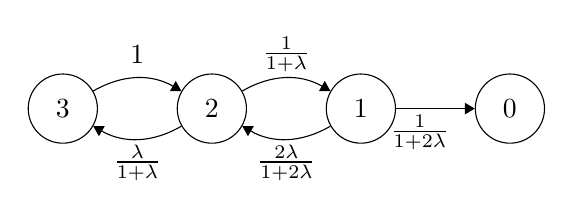
\begin{tikzpicture}[start chain = going right,
   -Triangle, every loop/.append style = {-Triangle}]
   \node[state, on chain]  (3) {3};
   \node[state, on chain]  (2) {2};
   \node[state, on chain]  (1) {1};
   \node[state, on chain]  (0) {0};
   
   \draw (3) edge[bend left] node[yshift=3mm]{$1$} (2);
   \draw (2) edge[bend left] node[yshift=-3mm]{$\frac{ \lambda}{1 + \lambda}$}(3);
   %
   \draw (2) edge[bend left] node[yshift=3mm]{$\frac{1}{1 + \lambda}$} (1);
   \draw (1) edge[bend left] node[yshift=-3mm]{$\frac{2\lambda}{1 + 2 \lambda}$}(2);
   %
   \draw (1) edge[left] node[xshift=3mm, yshift=-3mm]{$\frac{1}{1 + 2\lambda}$} (0);
   
\end{tikzpicture}
    \caption{Embedded discrete Markov chain for three node contact process}
    \label{fig:discrete_mc_three_contact}
\end{figure}

\subsubsection{Limiting Distribution}
\begin{theorem}
Let $T_\lambda$ be the time in which we hit 0 in the three node complete contact process.
Then $\frac{3}{2 \lambda^2 + \lambda + 1} T_\lambda$ converges in distribution to an exponential distribution with rate 1.
\end{theorem}

\begin{proof}
Again using Theorem \eqref{thm:geom_sum_exp}, we have that
\begin{align*}
    \sum_{i = 1}^{N_3} X_i^{(3)} &\sim \exp\left(
        \frac{3}{2\lambda^2 + \lambda + 1}
        \right) \\
    \sum_{i = 1}^{N_2} X_i^{(2)} &\sim \exp\left(
        \frac{2 + 2\lambda}{2 \lambda^2 + 3\lambda + 1}
    \right)\\
    \sum_{i = 1}^{N_1} X_i^{(1)} &\sim \exp\left(\frac{1 + 2\lambda}{1 + 2\lambda}\right)
\end{align*}

Multiplying $T_\lambda$ by $\frac{3}{2 \lambda^2 + \lambda + 1}$ and using Theorem \eqref{thm:exp_scaling}, we get
\begin{align*}
    \frac{3}{2 \lambda^2 + \lambda + 1} \sum_{i = 1}^{N_3} X_i^{(3)} &\sim \exp\left(
        1
        \right) \text{as } \lambda \to \infty\\
    \frac{3}{2 \lambda^2 + \lambda + 1} \sum_{i = 1}^{N_2} X_i^{(2)} &\sim \exp\left(
        \frac{(2 + 2\lambda)(2 \lambda^2 + \lambda + 1)}{3 (2 \lambda^2 + 3\lambda + 1)}
    \right)  \Rightarrow 0 \quad \text{as } \lambda \to \infty\\
    \frac{3}{2 \lambda^2 + \lambda + 1} \sum_{i = 1}^{N_1} X_i^{(1)} &\sim \exp\left(
    \frac{2 \lambda^2 + \lambda + 1}{3}
    \right) \Rightarrow 0 \quad \text{as } \lambda \to \infty
\end{align*}

So we have that $\frac{3}{2 \lambda^2 + \lambda + 1} T_\lambda$ converges in distribution to an exponential distribution with rate 1.
\end{proof}

\subsection{N node complete graph contact process}

\begin{figure}
    \centering
    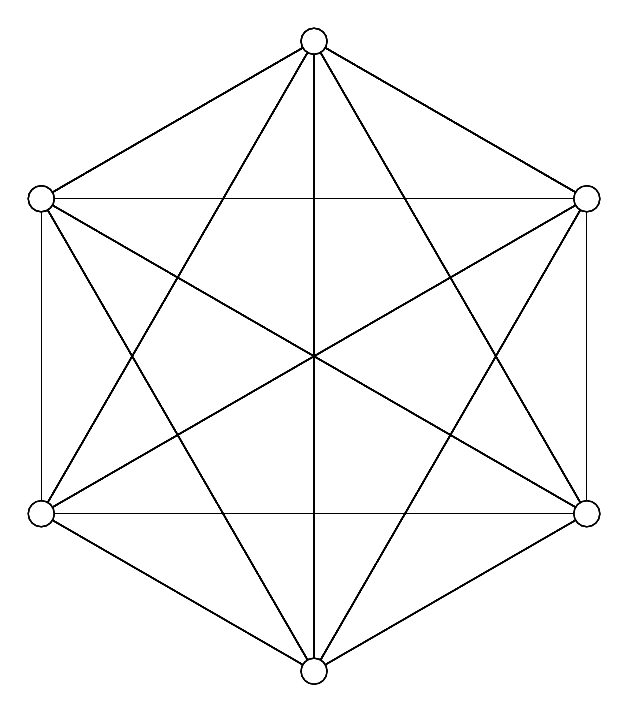
\begin{tikzpicture}
      \graph[circular placement, radius=4cm,
         empty nodes, nodes={circle,draw}] {
    \foreach \x in {a,...,z} {
      \foreach \y in {\x,...,f} {
        \x -- \y;
      };
    };
    };
    \end{tikzpicture}
    \caption{Complete graph N node contact process}
    \label{fig:n_nodes_contact}
\end{figure}

\begin{figure}
    \centering
   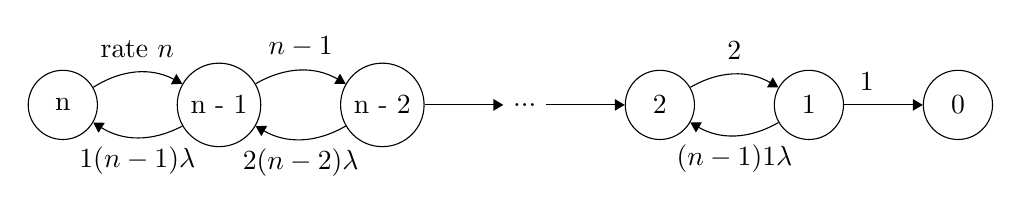
\begin{tikzpicture}[
   start chain = going right,
   -Triangle,
   every loop/.append style = {-Triangle}]
   \node[state, on chain]  (n) {n};
   \node[state, on chain]  (n1) {n - 1};
   \node[state, on chain]  (n2) {n - 2};
   \node[state without output/.append style={draw=none}, on chain]  (dots1) {...};
   \node[state, on chain]  (2) {2};
   \node[state, on chain]  (1) {1};
   \node[state, on chain]  (0) {0};
   
   \draw (n) edge[bend left] node[yshift=3mm]{rate $n$} (n1);
   \draw (n1) edge[bend left] node[yshift=-3mm]{$1 (n - 1) \lambda$}(n);
   
   \draw (n1) edge[bend left] node[yshift=3mm]{$n-1$} (n2);
   \draw (n2) edge[bend left] node[yshift=-3mm]{$2 (n - 2)\lambda$}(n1);
   
   \draw (n2) edge[left] node[xshift=3mm, yshift=-3mm]{} (dots1);
   
   \draw (dots1) edge[left] node[xshift=3mm, yshift=-3mm]{} (2);
   
  \draw (2) edge[bend left] node[yshift=3mm]{$2$} (1);
   \draw (1) edge[bend left] node[yshift=-3mm]{$(n - 1)1 \lambda$}(2);
   
  \draw (1) edge[left] node[yshift=3mm]{$1$} (0);
\end{tikzpicture}
    \caption{Transition rates for N node complete contact process}
    \label{fig:complete_contact_n_node_rates}
\end{figure}

In Figure \ref{fig:complete_contact_n_node_rates}, we show the transition rates for between the states of the contact process on the complete graph.
Note that for $i \in \{1, n - 1\} $ nodes that have a state of one, we have that the rate of going to $i + 1$ nodes is one of the $n - i$ nodes turning to one, each at a rate of $\lambda i$.
Thus, a total rate of $i (n - i) \lambda$.
The rate of going state with $i - 1$ ones is $i$ since we have $i$ nodes that have a potential to switch to zero, each with a rate of one.

Let $T_\lambda$ be the time until we reach state zero.
Now let $N_1, N_2, \ldots, N_m$ be the number of visits to states $1, 2, \ldots, m$ respectively.
Let $X_i^{(n)} \sim \exp(n)$ be iid random variables, $X_i^{(j)} \sim \exp(n - i + i(n - i)\lambda)$ for each $j \in \{1, \ldots, n-1\}$.
We can again represent $T_\lambda$ as random sums

\begin{equation}\label{eq:wait_contact_sum}
    T_\lambda = \sum_{i = 1}^{N_n} X_i^{(n)} + \sum_{i = 1}^{N_{n - 1}} X_i^{(n - 1)} + \cdots + \sum_{i = 1}^{N_1} X_i^{(1)}
\end{equation}

Since we are concerned with the limiting distribution we can instead focus on the rates up to a constant

\begin{theorem}
Let $N_k^{(n)}$ be a random variable that denoted the number of visits to state $k$ (that is, there are $k$ nodes with 1 with $n$ possible nodes) which is geometrically distributed. Then,
$$
E[N_k^{(n)}] = \begin{cases}
    O(\lambda^k) & k < n\\
    O(\lambda^{n - 1}) & k = n
\end{cases}
$$
\end{theorem}

\begin{proof}
We proceed by induction.
For the $k = 1$, we have that the parameter for $N_1^{(n)}$ is proportional to $\lambda$ since a success for the geometric distribution is going from state 1 to absorbing state 0.

Now assume that $k \not = n$ and will show it hold for $k + 1$.
Assume that $k + 1 \not = n$.
Then define geometric random variables $Y_1, Y_2, \ldots$ supported on $1,2,\ldots$ which denote the number of jumps from $k + 1$ to $k + 2$ before jumping to $k$.
Note that we do not care about what the system does after going to $k + 2$ since the state is guaranteed to return back to $k + 1$.
We have that $Y_i$ has a parameter proportional to $1/\lambda$.
Now let $M$ be another geometric random variable that represents the number of times that the process goes back to $k + 1$ from $k$.

It follows that
\begin{equation}
   N_{k + 1}^{(n)} = \sum_{i = 1}^M Y_i
\end{equation}

Then using Theorem \eqref{thm:geom_sum_geom}, we can conclude that $N_{k + 1}{(n)}$ is geometrically distributed with parameter proportional to $O(1/\lambda^{k + 1})$ or equivalently $N_{k + 1}{(n)} = O(\lambda^{k + 1})$

We can use the same reasoning for the case when $k = n$ case if we let $M$ have parameter 1 (since we always go to state $n - 1$), then it follows that $E[N_{n}{(n)}] = O(\lambda^{n - 1})$
\end{proof}

\begin{theorem}
Let $T_\lambda$ be the waiting time until we reach state 1 in the $n$ node complete contact process.
The limiting distribution of $O(1/\lambda^{n - 1}) \cdot T_\lambda$ is an exponential distribution with parameter 1.
\end{theorem}

\begin{proof}
If we multiply Equation \eqref{eq:wait_contact_sum} by $O(1/\lambda^{n - 1})$ then for each $k < n$, by Theorem \eqref{thm:geom_sum_exp}, \eqref{thm:exp_scaling}, $O(1/\lambda^{n - 1}) \sum_{i = 
1}^{N_{k}} X_i^{(k)}$ will have a exponential distribution with parameter proportional to $O(\lambda^{n - k - 1})$ which approaches zero in distribution as $\lambda \to \infty$.

For $k = n$, we have that
$$
O(1/\lambda^{n - 1}) \sum_{i = 
1}^{N_{n}} X_i^{(n)} \Rightarrow \exp(1)
$$
as $\lambda \to \infty$.
\end{proof}

\section{Finite contact process on 1D lattice}

The two node contact process on the lattice is identical to the complete graph.

\subsection{Three node contact process}

For the three node contact process, shown in Figure \ref{fig:three_node_contact_lattice} we have a transition graph shown in Figure \ref{fig:three_node_contact_lattice_states}.
Nodes 110 and 011 are combined due to symmetry as well as 100 and 001.


\begin{figure}
    \centering
   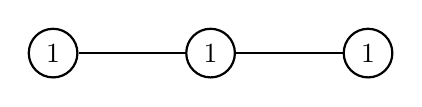
\begin{tikzpicture}[auto, node distance=2cm, every loop/.style={}, thick,main node/.style={circle,draw}]
   \node[main node]  (0) {1};
   \node[main node]  (1) [right of=0]  {1};
   \node[main node]  (2) [right of=1]  {1};
   
   \draw (0) edge [left] (1);
   \draw (1) edge [left] (2);
\end{tikzpicture}
    \caption{Three node contact process on 1D lattice}
    \label{fig:three_node_contact_lattice}
\end{figure}

\begin{figure}
    \centering
   %\begin{tikzpicture}[auto, node distance=2cm, every loop/.style={-Triangle}, thick,main node/.style={circle,draw}]
  \begin{tikzpicture}[start chain = going right,
   -Triangle, every loop/.append style = {-Triangle}]
   \node[state, on chain]  (111) {111};
   \node[state, on chain]  (110) [above right of=111, yshift = 4mm]  {110};
   \node[state, on chain]  (101) [below right of=111, yshift = -4mm]  {101};
   
   \node[state, on chain]  (010) [right of=110, xshift=3mm]  {010};
   \node[state, on chain]  (100) [right of=101, xshift=3mm]  {100};
   
   \node[state, on chain]  (000) [below right of=010]  {000};
   
   
   \draw (111) edge [bend left] node[yshift=3mm]{$2$} (110);
   \draw (110) edge [] node[yshift=-2mm, xshift=1.5mm]{$\lambda$} (111);
  
   \draw (111) edge [bend right] node[yshift=-3mm]{$1$} (101);
   \draw (101) edge [] node[yshift=1.5mm, xshift = 2mm]{$2\lambda$} (111);
    
   \draw (110) edge [bend left] node[yshift=3mm]{$1$} (010);
   \draw (010) edge [] node[yshift=-2mm, xshift=1.5mm]{$2 \lambda$} (110);
  
   \draw (101) edge [] node[yshift=-3mm]{$2$} (100);
   
   \draw (110) edge [] node[yshift=3mm]{$1$} (100);
   \draw (100) edge [bend left] node[yshift=3mm]{$\lambda$} (110);

  \draw (010) edge [] node[yshift=3mm]{$1$} (000);
  \draw (100) edge [] node[yshift=-3mm]{$1$} (000);
    
\end{tikzpicture}
    \caption{Three node contact process rates between each states}
    \label{fig:three_node_contact_lattice_states}
\end{figure}


\subsection{Voter Model}

\bibliographystyle{plainnat}
\bibliography{references}
\end{document}
